%%%%%%%%%%%%%%%%%%%%%%%%%%%%%%%%%%%%%%%%%
% University Assignment Title Page 
% LaTeX Template
% Version 1.0 (27/12/12)
%
% This template has been downloaded from:
% http://www.LaTeXTemplates.com
%
% Original author:
% WikiBooks (http://en.wikibooks.org/wiki/LaTeX/Title_Creation)
%
% License:
% CC BY-NC-SA 3.0 (http://creativecommons.org/licenses/by-nc-sa/3.0/)
% 
% Instructions for using this template:
% This title page is capable of being compiled as is. This is not useful for 
% including it in another document. To do this, you have two options: 
%
% 1) Copy/paste everything between \begin{document} and \end{document} 
% starting at \begin{titlepage} and paste this into another LaTeX file where you 
% want your title page.
% OR
% 2) Remove everything outside the \begin{titlepage} and \end{titlepage} and 
% move this file to the same directory as the LaTeX file you wish to add it to. 
% Then add \input{./title_page_1.tex} to your LaTeX file where you want your
% title page.
%
%%%%%%%%%%%%%%%%%%%%%%%%%%%%%%%%%%%%%%%%%
%\title{Title page with logo}
%----------------------------------------------------------------------------------------
%	PACKAGES AND OTHER DOCUMENT CONFIGURATIONS
%----------------------------------------------------------------------------------------

\documentclass[11pt]{article}
\usepackage[english]{babel}
\usepackage[utf8x]{inputenc}
\usepackage{amsmath}
\usepackage{fancyhdr}
\usepackage{graphicx}
\usepackage[colorinlistoftodos]{todonotes}
\usepackage{geometry}
\pagestyle{fancy}
\geometry
{
 a4paper,==
 total={170mm,257mm},
 left=20mm,
 top=20mm,
}
\fancyheadoffset{0.1cm}
\lhead{Mingyang Zhang : 650242, Shreyash Patodia : 767336}
\rhead{mingyangz, spatodia}



\begin{document}

\section{Introduction}


In this assignment we were asked to classify instances in the Abalone Dataset into one of two 
('young' or 'old') or three ('very young', 'old' and 'middle-age') categories. The classification method meant to be used was K-Nearest Neighbours. We could choose our similarity metrics, voting methods, evaluation methods and also the validation framework for the dataset. Our choices are listed below:
\\\\
{\centering
\begin{tabular}{|p{3.5cm}||p{3.5cm}|p{3.5cm}|p{3.75cm}|}
 \hline
 {\bf Similarity Metric} & Euclidean Distance & Manhattan Distance & Minkowski Distance (with p = 0.5)\\
 \hline
 {\bf Voting Method} & Equality Weight Majority & Inverse Distance & Inverse Linear Distance \\ 
 \hline
 {\bf Evaluation Metric} & Accuracy and Error & Precision & Recall \\ 
 \hline
\end{tabular} }
\\\\ \\
For our validation framework we use {\bf 10-Fold Cross Validation} (but also, implement holdout). 

 

\section{Similarity Metrics}

\subsection{Euclidean, Manhattan and Minkowski - as good choices}

The Abalone dataset contains eight attributes out of which 7 are of a continuous nature, so it made sense to us to use some sort of distance metric to evaluate similarity instead of checking for equality  (like for Jaccard and Dice Similarity) or something like cosine similarity, which would compare the angles between the abalones and would assign high similarity to abalones with similar proportions but with very different sizes (and thus, possibly different ages as living being grow). If p and q are the instances to be compared the formula for our similarity metrics are: \\

Euclidean Distance:
\begin{equation}
\sqrt{\sum_{i=1}^{n} (p_{i} - q_{i})^{2}}
\end{equation}

Manhattan Distance:
\begin{equation}
\sum_{i=1}^{n} |p_{i} - q_{i}|
\end{equation}

Minkowski Distance:
\begin{equation}
{(\sum_{i=1}^{n} {|p_{i} - q_{i}|}^{pow})}^{1/pow}
\end{equation}
\\
(We take pow = 0.5 for Minkowski distance, as it lets makes for a nice comparison with Euclidean. {\bf when we refer to Minkowski in this report we will talk about the specific case with pow = 0.5}) \\

Euclidean takes sum of squares before finding the root, Manhattan is plain addition of distances values and Minkowski (with p = 0.5) takes the root of each value before summing them up and squaring the sum. We especially wanted to contrast Minkowski and Euclidean since Minkowski is actually going to amplify larger distances (since most distances are less than 1) and Euclidean would tend to suppress it by squaring (square of number less than 1 is less than the number itself). 


\subsection{Euclidean - as the best}

Our choices of Euclidean, Minkowski (p = 0.5) and Manhattan Distance all of which find the distances in values of attributes for instances would give similar results with this dataset due to the values of distances being in a relatively small range but we conducted some experiments to determine which one is the "best". The experiments (results in Table 1) show us that that the performance of all of the similarity metrics is very closely lumped together (as expected), but Euclidean seems to be slightly more accurate and have higher precision/recall so we consider it to be the "best" for this dataset.

(Note: All measurements in the tables are averages of 10 runs with 10 fold cross validation)

\begin{table}[h]
\centering
\begin{tabular}{|p{2cm}|p{3cm}||p{2cm}|p{1.5cm}|p{1.5cm}|p{1.5cm}|}
 \hline
 \multicolumn{6}{|c|}{Similarity Experiment} \\
 \hline
 Dataset & Parameters & Similarity Metric & Accuracy & Precision & Recall\\
 \hline
 Abalone-3 & k=29,voting=inv. distance &   euclidean & 0.7676  & 0.6469 & 0.6487\\
 \hline
 Abalone-3 & k=29,voting=inv. distance &   minkowski & 0.7663 & 0.6468 & 0.6473\\
 \hline
 Abalone-3 & k=29,voting=inv. distance &   manhattan & 0.7641 & 0.6420 & 0.6436\\ 
 \hline
 Abalone-2 & k=29,voting=inv. distance &   euclidean & 0.7857  & 0.7714 & 0.7399\\
 \hline
 Abalone-2 & k=29,voting=inv. distance &   minkowski & 0.7787 & 0.7654 & 0.7299\\
 \hline
 Abalone-2 & k=29,voting=inv. distance &   manhattan & 0.7830  & 0.7683 & 0.7355\\ 
 \hline

\end{tabular}
\caption{Table of experiments with different similarity metric}
\end{table}
\label{Figure 1}


% Commands to include a figure:
%\begin{figure}[!htb]
%\centering
% \includegraphics[width=0.5\textwidth]{BadExample.png}
% \caption{\label{fig:frog}Bad Design Example}
%\end{figure}


\section{Validation Framework}

\subsection{M-Fold Cross Validation}

For our validation framework we used 10-Fold Cross Validation, we first divide the dataset into 10 (approximately) equal partitions and then perform K-Nearest Neighbour classification by choosing each of the 10 partitions as our test set (and the amalgamation of the remaining 9 as our training set) for one run of the K-Nearest Neighbour algorithm. This leads to very stable evaluation measures across different runs of out program since performing the algorithm 10 times means that any positive outlier is (very likely to be) averaged out by negative ones. In our strategy, if the dataset cannot be divided into partitions of equal sizes then we just keep on adding one instance to the partitions (starting at the 0th partition) until there are no instances remaining.\\

We tested 10-Fold Cross Validation against holdout (split at 90:10), 5-Fold Cross Validation and 20-Fold Cross Validation and here are graphs of their accuracies for 10 different runs with Abalone-2 and Abalone-3 each (here k=29, similarity=euclidean and voting=inverse distance):


% Commands to include a figure:
%\begin{figure}[!htb]
%\centering
% \includegraphics[width=0.5\textwidth]{BadExample.png}
% \caption{\label{fig:frog}Bad Design Example}
%\end{figure}

\begin{figure}[!htb]
\centering

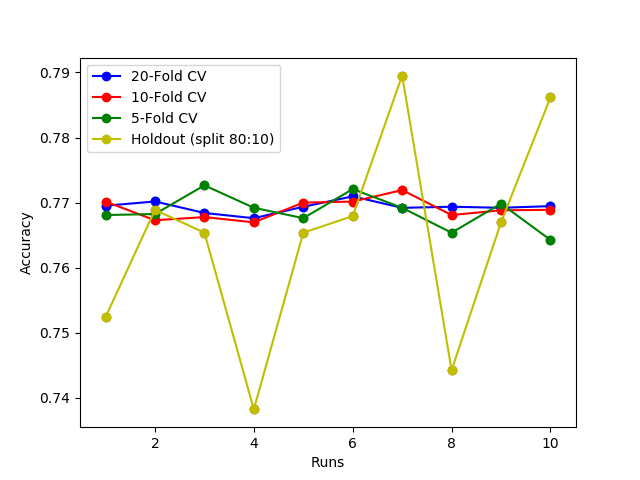
\includegraphics[width=0.5\textwidth]{consistency_comparison_3.png}
\caption{Comparison of the consistency of the accuracy of prediction over multiple runs of different validation methods with Abalone-3}
\end{figure}

\begin{figure}[!htb]
\centering

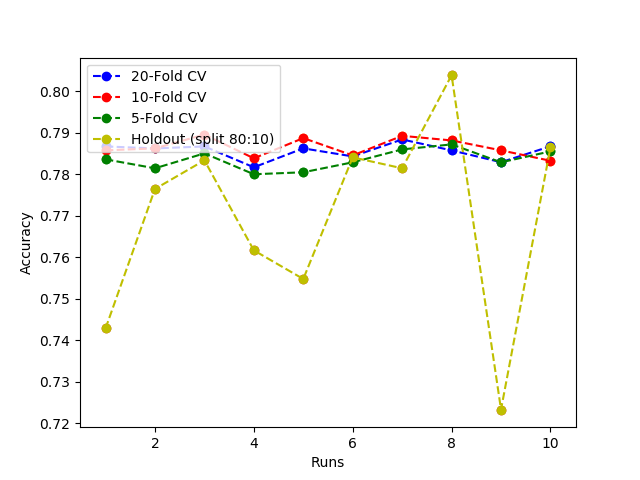
\includegraphics[width=0.5\textwidth]{consistency_comparison_2.png}
\caption{Comparison of the consistency of the accuracy of prediction over multiple runs of different validation methods with Abalone-2}
\end{figure}


From the above graphs it is clear that cross-validation is far more consistent in terms of predictive accuracy than holdout (similar plots were observed for precision and recall but the plots were not included for conciseness). We also, see using 5 folds is more variable than using 10 or 20 folds potentially because it has less training data. 10 and 20 fold have similar results but we chose 10 folds since it allows for more test data (thus, more test coverage) and is also a standard M for cross validation. 


\section{Representation of Data}

We are using a 2-tuple to represent the dataset wherein the first element of the tuple is the list of instances and the second element of the dataset is the list of class labels. Our data is normalized using formula (4), in order to make sure that Euclidean distance does not under-estimate the similarity of some types of instances:
\\
\begin{equation}
x_i = x_i/(\sqrt{\sum_{i=1}^{n} x_i^2}) \text{, where } x_i \text{ is an attribute of the instance } x
\end{equation}
\\
In our pre-processing of the data we determined that it was best to work with {\bf all of the attributes other than the gender} (we also tried removing some attributes during post-processing and seeing results but results were best when we used all of the continuous attributes). We chose to remove gender from the reckoning because in order to use gender in our similarity metrics we had to do some sort of transformation to numerical values which was not guaranteed to be ideal. Moreover, our results show that including gender lead to a decrease in accuracy, precision and recall (average over 10 runs of each). For example:

\begin{table}[h]
\centering
\begin{tabular}{|p{2cm}|p{4cm}||p{2cm}|p{1.5cm}|p{1.5cm}|p{1.5cm}|}
 \hline
 \multicolumn{6}{|c|}{Similarity Experiment} \\
 \hline
 Gender Included & Parameters & Similarity Metric & Accuracy & Precision & Recall\\
 \hline
 No & k=29,voting=inverse distance &   euclidean & 0.7676  & 0.6469 & 0.6487\\
 \hline
 Yes & k=29,voting=inverse distance &   euclidean & 0.7542 & 0.6334 & 0.6373\\
 \hline
 No & k=29,voting=inverse distance &   manhattan & 0.7641 & 0.6420 & 0.6436\\ 
 \hline
 Yes & k=29,voting=inverse distance &  manhattan & 0.7531  & 0.6314 & 0.6452\\
 \hline
 No & k=29,voting=inverse distance &   minkowski & 0.7616 & 0.6291 & 0.6289\\
 \hline
 Yes & k=29,voting=inverse distance &   minkowski & 0.7578  & 0.6221 & 0.6219\\ 
 \hline
 No & k=29,voting=majority vote &   euclidean & 0.7631  & 0.6293 & 0.6321\\
 \hline
 Yes & k=29,voting=majority vote &   euclidean & 0.7564 & 0.6227 & 0.6287\\
 \hline
 No & k=29,voting=majority vote &   manhattan & 0.7626 & 0.6312 & 0.6156\\ 
 \hline
 Yes & k=29,voting=majority vote &  manhattan & 0.7539  & 0.6247 & 0.6128\\
 \hline
 No & k=29,voting=majority vote &   minkowski & 0.7610 & 0.6301 & 0.6245\\
 \hline
 Yes & k=29,voting=majority vote &   minkowski & 0.7512  & 0.6234 & 0.6178\\ 
 \hline

\end{tabular}
\caption{Table of experiment for different test scenarios with or without including gender, tests were run for Abalone-3}
\end{table}

We also found that height and whole weight are very low for abalones with label "very-young" and is quite a bit higher for older abalones, so we decided to scale these two attributes by a factor of 2 to make this difference more pronounced. This lead to an increase in accuracy, precision and recall by around 2\%. This step was taken on the basis of observations from the dataset, while trying to find the 
attributes that separate the classes. The multiplication is done pre-normalization to not make sure we don't go past the bounds of normalization. 



\subsection{A good value of k}

After a bit of research we found that it was common to choose k as the square root of the number of instances in the dataset, so we conducted an experiment by varying k to be the prime numbers between 3-100 (so around the square root) to get the best value. The experiments were conducted to maximize accuracy without compromising on precision and recall (we ended up getting pretty high values for all 3). The results of the experiments are: 

\begin{figure}[!htb]
\centering

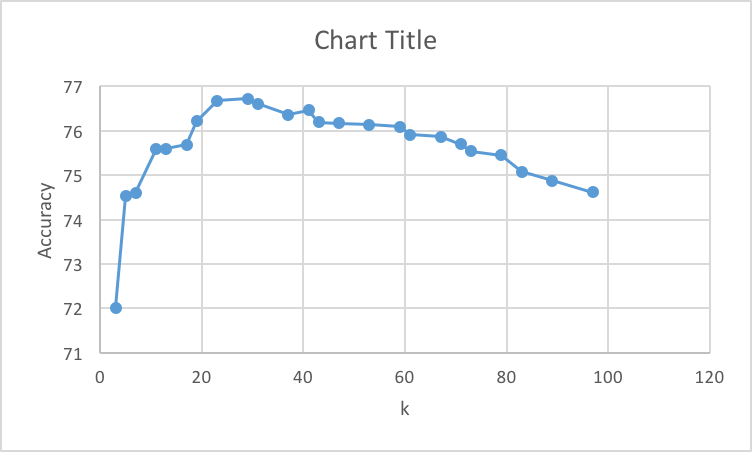
\includegraphics[width=0.5\textwidth]{k_accuracies_3.png}
\caption{Plot of Accuracy vs k-values for Abalone-3}
\end{figure}

\begin{figure}[!htb]
\centering

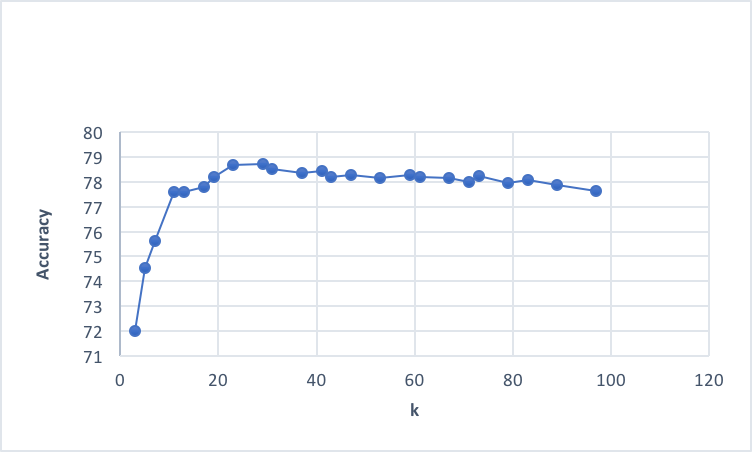
\includegraphics[width=0.5\textwidth]{k_accuracies_2.png}
\caption{Plot of Accuracy vs k-values for Abalone-2}
\end{figure}

We see that for k around 29 we get a peak, and we chose that as our default value of k, the accuracy drops off towards k=100 since we probably start getting a bias towards the majority class. 




\section{Our voting methods}

We implemented three voting methods, one that just counts the majority class amongst the neighbours of the test instance i.e. {\bf equal weight}, the other two are: 
\\\\
Inverse Distance: 
\begin{equation}
w_j = 1/(d_j + 0.5)  
\end{equation}
\\
Inverse Linear Distance:
\begin{equation}
w_j = 
\begin{cases}
    (d_k - d_j)/(d_k - d_1),& \text{where } d_k \text{ is the farthest neighbour, }  d_1 \text{ is the closest and } d_j \neq d_1\\
    1,              &  d_j = d_1 
\end{cases}
\end{equation}

Our experiments show that all voting methods work equally well with {\bf equal weight} surprisingly getting the ever so slightly better results. (See Table 3 for results)

\begin{table}[h]
\centering
\begin{tabular}{|p{2cm}|p{4.5cm}||p{2cm}|p{1.5cm}|p{1.5cm}|p{1.5cm}|}
 \hline
 \multicolumn{6}{|c|}{Similarity Experiment} \\
 \hline
 Dataset & Parameters & Voting Method & Accuracy & Precision & Recall\\
 \hline
 Abalone-3 & k=29,distance = euclidean &   equal weight & 0.7666  & 0.6467 & 0.6478\\
 \hline
 Abalone-3 & k=29,distance = euclidean & inverse distance & 0.7636 & 0.6417 & 0.6425\\
 \hline
 Abalone-3 & k=29,distance = euclidean &  inverse linear distance & 0.7612 & 0.6378 & 0.6390\\ 
 \hline

\end{tabular}
\caption{Table of experiments with different voting methods (avg. over 10 runs)}
\end{table}

\section{Our evaluation methods}

We implement functions to calculate Accuracy, Precision and Recall (we {\bf macro-average} the Precision and Recall, so as to not give higher a weight to the majority class and overshadow the others). We also implement a function to find the error using the accuracy. In order to judge our performance we used the {\bf Zero-R} majority class voting rule as the baseline which has an accuracy of 0.65 and we comfortably beat it with an accuracy of 0.78 on average for Abalone-2. For Abalone-3, the Zero-R method gives us a baseline accuracy of around 0.35 and our program clears that without too many issues. But for Abalone-3 our program struggles to find "middle-age" abalones as compared to "very-young" and "old" ones, probably because there isn't much difference in the values of the attributes for "old" and "middle-age" abalones (thus, greatly affection our recall and precision). {\bf Answer to challenge question:} Division in Abalone-2 was done in such a way that baseline is not too easy to beat, and Abalone-3 was divide equally so that if our classifier predicts the majority class then it would have really bad performance for Abalone-3. 

\end{document}